\documentclass[12pt]{article}
\usepackage[utf8]{inputenc}

\usepackage{geometry}
\usepackage{setspace}
\usepackage{amsmath}
\usepackage[margin=1cm]{caption}
\usepackage{titling}
\usepackage{parskip}
\usepackage{booktabs}

\geometry{margin=.95in}
\onehalfspacing

\title{A decentralized insurance and reinsurance marketplace\\\vspace{5mm}\small\textit{V0.3}\vspace{20mm}}
\author{\textbf{Authors}\\Stephan Karpischek\\Christoph Mussenbrock\\Jake Brukhman\\Ron Bernstein\\\\\textbf{Reviewed by:}\\Chris Padovano\\Aleksandr Bulkin\\Alexander Felix\\\\}
\date

\usepackage{natbib}
\usepackage{graphicx}
\usepackage{titling}
\usepackage{float}
\usepackage{graphicx}
\graphicspath{ {images/} }
\usepackage{tocloft}
\usepackage{cals}

\pretitle{%
  \vspace{20mm}
  \begin{center}
  \LARGE
  
\includegraphics[scale=.3]{etherisc}\\
}
\posttitle{\end{center}}

\begin{document}

%
% TITLE
%
\maketitle
\newpage
\begin{figure}[H]
    \vspace{30mm}
    \begin{center}
        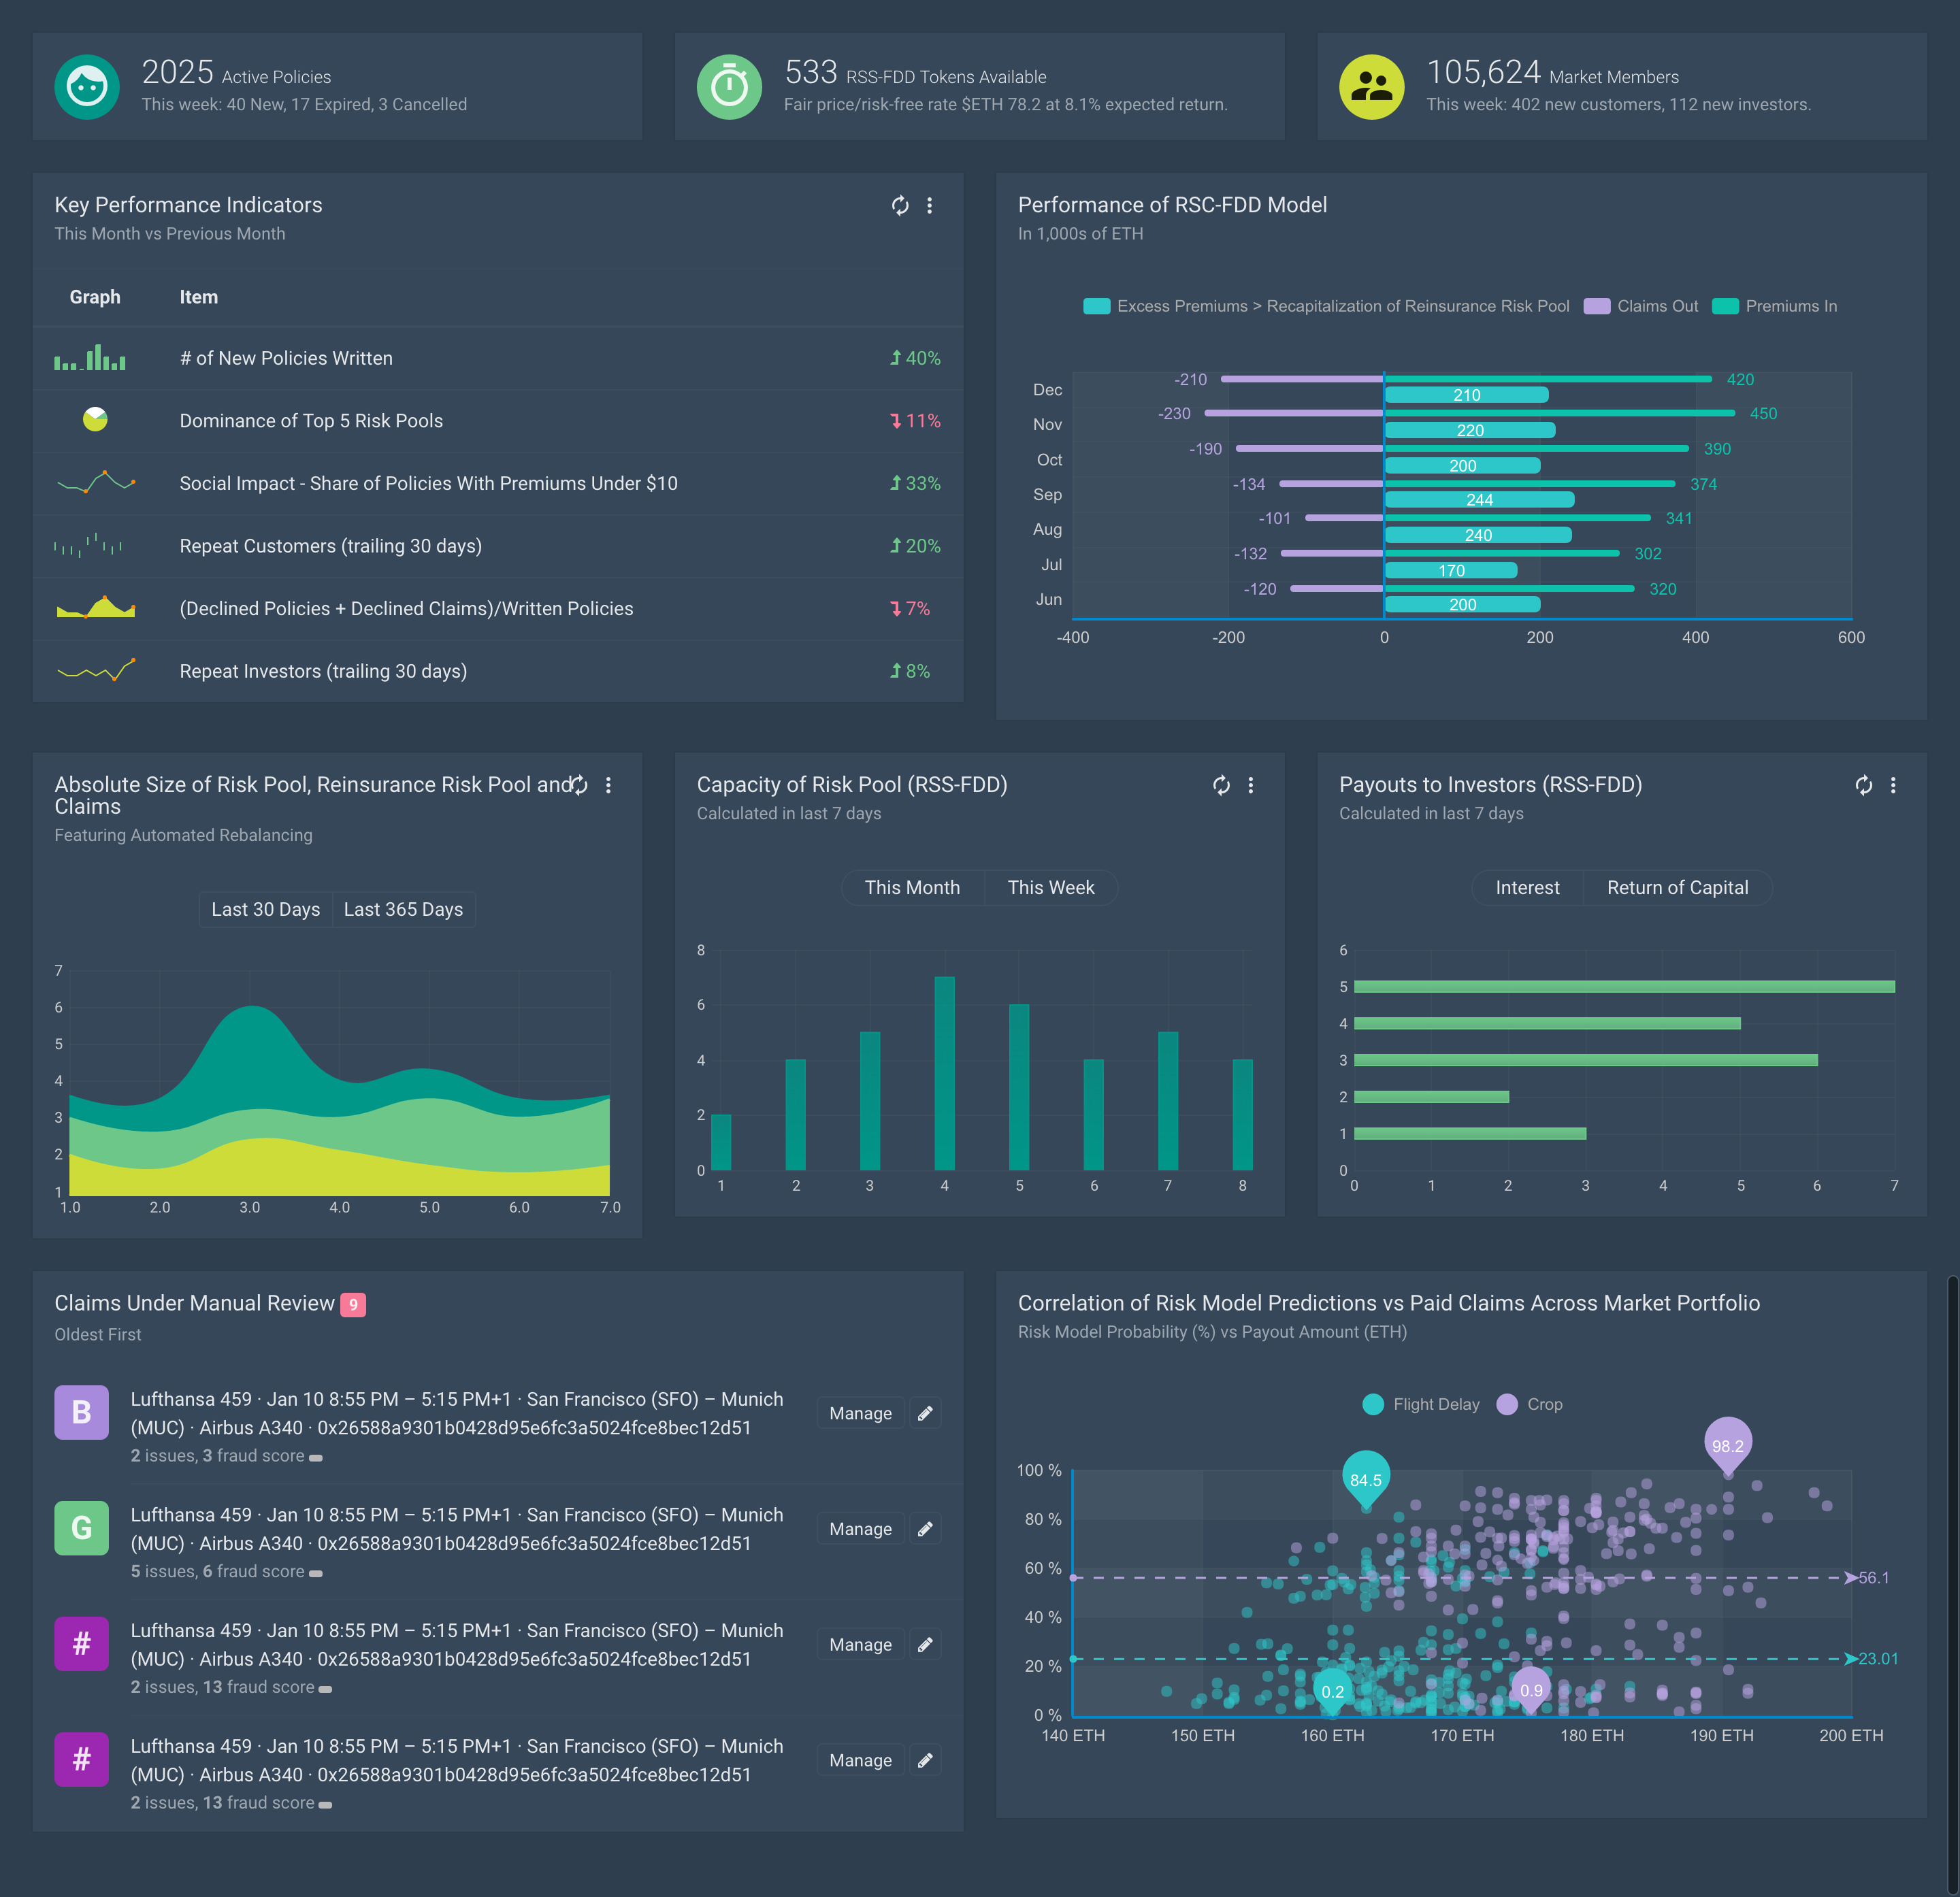
\includegraphics[scale=.15]{etheriscbeta}
    \end{center}
    \caption{\footnotesize Mockup for the Etherisc dashboard.}\label{fig1}
\end{figure}
\newpage

%
% TOC
%
\renewcommand{\cftsecleader}{\cftdotfill{\cftdotsep}}
\tableofcontents
\newpage

%
% DISCLAIMER
%
\section{Disclaimer}

All of the information presented in this whitepaper is tentative and is subject to change at any time. None of the information herein should be construed as legal, accounting, or investment advice of any kind. This document does not represent a solicitation for investment, nor does it represent an offering or sale, public or private, of any kind of financial instrument, security or otherwise, in any jurisdiction. This whitepaper is provided as-is, for informational purposes only, with the intention of describing a prospective software system.

\newpage

\section{Abstract}

Etherisc's mission is to build decentralized insurance applications, making the purchase and sale of insurance more efficient, enable lower operational costs, provide greater transparency into the industry of insurance compared to traditional operations, and democratize access to reinsurance investments.  

In September 2016, we created and alpha-tested a parametric insurance application for consumers. The Flight Delay Dapp\footnote{https://fdd.etherisc.com/} successfully demonstrated the benefits of decentralized insurance by providing flight delay insurance policies to attendees of Ethereum's Devcon2 conference held in Shanghai, China. The risk pool for this demonstration was capitalized by the Etherisc team and, though limited in size, clearly demonstrated an innovative decentralization use case worthy of further exploration.

Based on our research and experience with the Flight Delay Dapp, it is clear that insurance applications with fixed risk pools do not scale. Cryptographic tokens enable highly customized economics. Our goal is to tokenize reinsurance risks and make them available on a global “open access” marketplace . This strategy provides both flexibility and scale for decentralized insurance risk pools, enables new types of insurance products, makes the product extremely safe for customers, and democratizes access to reinsurance investments.

In this whitepaper, we propose an end-to-end decentralized insurance product and a reinsurance marketplace on the Ethereum blockchain as our contribution to hack.ether.camp. We present a token model which enables investors to buy and trade the “long-tail” risks of a decentralized insurance portfolio and to gain exposure to its revenue as an income stream. Together with a consumer-facing insurance application, this forms a complete and fully functioning “trustless” insurance system on the blockchain.

Our strategy is to start with a simple use case and flight delay insurance is a natural candidate which has some desirable properties: individual risks are small and relatively independent and claim verification can be fully automated. 

Our work with flight delay insurance will be a starting point to build upon and further expand into other insurance verticals and completely new insurance products. The prototype will provide the necessary building blocks to create the future of insurance on the blockchain.

%%
%% VISION & STRATEGY
%%

\section{Vision \& Strategy}

\subsection{Motivation}

The insurance market is dominated by large, traditional players including institutional underwriters, brokers, and resellers. Insurance companies act as intermediaries between protection seekers who want to share some risk on one side and investors who provide capital to cover risks on the other side. In return for the provision of capital investors get access to an insurance-backed asset class.

Insurance companies are highly centralized and hierarchical organizations with much longer software development lifecycles than modern technology companies. At the same time, it is challenging for new competitors to enter the market because of strong network effects: insurance is a big numbers game, and this gives incumbents strong statistical and marketing advantages. Tight regulation and entrenched interests have allowed the industry to resist business model disruption for many years.

As a highly automatable platform for efficient custom economics systems, blockchain technology is well-suited to disrupt the insurance industry. With the advent of decentralized smart contract platforms there is now sufficiently mature technology for viable end-to-end digital insurance solutions and thus disintermediation of these markets. We foresee that blockchain technology will impact insurance products in the following core areas:

\begin{enumerate}
    \item \textbf{Efficiency and Automation.} Smart contract technology enables end-to-end automation of payments, efficient risk model estimation, and semi-automated claims processing, thus substantially lowering operating costs.

    \item \textbf{Access for Insurance Customers.} Lower costs enable insurance solutions for developing markets, low-income businesses, and new product verticals which have been previously unable to obtain insurance. For example, crop insurance for rural farmers in developing countries is an underserved market and a good candidate for further exploration.

    \item \textbf{Access for Insurance Investors.} Digital assets on blockchains create opportunities to structure exposure to insurance products for a much broader range of investors. 

    \item \textbf{Transparency.} On most blockchains, transparency is a platform-level feature. All data in a smart contract based system is publicly auditable and can be freely analyzed by third parties. Etherisc will also provide a user friendly, comprehensive frontend displaying the key performance indicators of the system. 
\end{enumerate}

Finally, we posit that the availability of insurance products via blockchain and distributed ledger technologies will reinforce the adoption of digital currencies and decentralized business models, creating beneficial network effects for insurance products themselves.

\subsection{Scope}

At Etherisc, we're aiming for a Minimum Loveable Product (MLP)\footnote{https://medium.com/the-happy-startup-school/} which consists of an automated smart contract for issuing and claiming insurance policies, an automated reinsurance market based on cryptographic tokens, a risk management economic model with transparent and aligned incentives for participants, and a great user experience. The details of the components of the Etherisc MLP may be found in Section \ref{architecture} section below.

We will start our project with a simple model based on the Flight Delay Dapp. Flight delays are a natural use-case for parametric insurance\footnote{https://www.wikiwand.com/en/Parametric\_insurance}, that is, an insurance for which a damage and claim can be programmatically verified using a trusted data source. In this use case, the delay of each flight can be determined by requesting data from an online service, such as flightstats.com. The Flight Delay Dapp is a well-understood and thoroughly tested application which can issue policies and pay valid claims completely autonomously. Read more about our experience and lessons learned\footnote{https://medium.com/the-future-requires-more/flight-delay-dapp-lessons-learned-a59e4e39a8d1} from the Flight Delay Dapp experiment.

The logical next step is to add a token model to enable the risk-taking investor side of the reinsurance market. Tokens will flexibly adapt in real time to market demand and investor interest. The model will be self-adjusting and self-regulating, providing a solid base for a truly decentralized insurance model.

Part of the MLP will also be an intuitive, user-friendly frontend for both customers and investors, which will combine ease of access with full transparency.

%%
%% ROADMAP
%%

\section{Roadmap}

\subsection{Hackathon Milestones}

We aim to achieve the following milestones in the course of hack.ether.camp Virtual Accelerator:

\vspace{10mm}

\begin{center}
\begin{calstable}
\colwidths{{7cm}{7cm}}
\large
\brow 
    \cell{\textbf{Milestone}} 
    \cell{\textbf{Due Date/Period}} 
\erow
\normalsize
\brow 
    \cell{White paper draft version v0.1\\with first specification of risk pool and token model.}
    \cell{Friday, 16 December 2016}
\erow
\brow 
    \cell{White paper review and discussion}
    \cell{Friday, 16 December 2016 to\\
            Wednesday, 21 December 2016}
\erow
\brow 
    \cell{First implementation of risk pool and token contract, release on testnet}
    \cell{Tuesday, 20 December 2016}
\erow

\brow 
    \cell{White paper v0.2+ with reviewed\\token model}
    \cell{Thursday, 22 December 2016}
\erow

\brow 
    \cell{Python simulation demonstrating\\statistical model calculation}
    \cell{Thursday, 22 December 2016}
\erow


\end{calstable}
\end{center}

\subsection{Timeline For hack.ether.camp Funds}

The hack.ether.camp DST contract defines the following timeline:

\vspace{10mm}

\begin{center}
\begin{calstable}
\colwidths{{7cm}{7cm}}
\large
\brow 
    \cell{\textbf{Event}} 
    \cell{\textbf{Date/Period (GMT)}} 
\erow
\normalsize
\brow 
    \cell{
Start of the hackathon
}
    \cell{Thursday, 17 November 2016 14:00}
\erow
\brow 
    \cell{End of the hackathon; token sale for HKG ends; up to 5X sold tokens issued and offered for ETH.}
    \cell{Thursday, 22 December 2016 14:00}
\erow
\brow 
    \cell{First proposal can be submitted 8\\weeks after the event ends}
    \cell{Thursday, 16 February 2017 14:00}
\erow

\brow 
    \cell{Objection period ends after 	10 days, 20\% of funds can be released}
    \cell{Sunday, 26 February 2017 14:00}
\erow

\brow 
    \cell{One proposal for 20\% of funds every 2 weeks}
    \cell{Thursday, 2 March 2017 to\\Thursday, 13 April 2017}
\erow
\end{calstable}
\end{center}


\subsection{General Cost Estimates}

The Etherisc team estimates the following costs for the initial development of an MLP, broken down into the following areas:

\begin{itemize}
    \item \textbf{Research.} This includes research in mathematics, statistical and actuarial models, and computational simulations that will drive effective insurance models for Etherisc products.

    \item \textbf{Development.} This will include software development, smart contract development and security review, and developing user experience.

    \item \textbf{External Costs.} These will include token sale structure, security audits, legal advisory, bug bounties, and other fixed costs associated with product development.
\end{itemize}

The following table gives an overview of expected costs and an approximate breakdown of costs and deliverables according to different funding levels we hope to reach.
\vspace{10mm}
\begin{center}

\begin{figure}[H]
\centering
\textbf{Cost Estimates}\par\vspace{10mm}
\begin{calstable}
\colwidths{{4cm}{4.33cm}{4.33cm}{4.33cm}}
\large
\alignC
\brow 
    \cell{\textbf{Funding\vspace{3mm}}} 
    \cell{\textbf{Research}}
    \cell{\textbf{Development}}
    \cell{\textbf{Other}}
\erow
\alignL
\footnotesize
\brow 
    \cell{\textbf{\$12,500}}
    \cell{\$5,000}
    \cell{\$5,000}
    \cell{\$2,500}
\erow
\brow 
    \cell{\textit{(Current financing:\\approx. \$20,000)}}
    \cell{
        Build a simulator for Flight Delay;\\
        Acquire external data for FlightDelay;\\
        Run basic simulations
    }
    \cell{
    Build a simple demonstrator (frontend/backend);\\
    Deploy on testnet not ready for production
    }
    \cell{
        Basic audit on the mathematical model\\
        Prepare token sale
    }
\erow
\brow 
    \cell{\textbf{\$30,000}}
    \cell{\$10,000}
    \cell{\$15,000}
    \cell{\$5,000}
\erow
\brow 
    \cell{}
    \cell{
        Develop a concept for continuous validation & backtesting of system
    }
    \cell{
        Build a functional and complete DApp, simple UI;\\
        Backend with contracts \& investor side
    }
    \cell{
        As above
    }
\erow

\brow 
    \cell{\textbf{\$70,000}}
    \cell{\$20,000}
    \cell{\$30,000}
    \cell{\$20,000}
\erow

\brow 
    \cell{}
    \cell{
    Extend mathematical\\model;\\
    Include correlation and\\further data sources, such as weather \& airport data
    }
    \cell{
        MLP;\\
        Build a great UX/UI;\\
        Small scale deployment\\ possible
    }
    \cell{
        Legal and regulatory\\framework;\\
        Campaign for token sale;\\
        Legal audit for token sale
    }
\erow

\brow 
    \cell{\textbf{\$100,000}}
    \cell{\$30,000}
    \cell{\$40,000}
    \cell{\$30,000}
\erow

\brow 
    \cell{}
    \cell{
        Finished model
    }
    \cell{
        MLP;\\
        Testing and refined UX/UI;\\
        Production ready for larger scale
    }
    \cell{
        Thorough audit on mathematical and actuarial model;\\
        Security audits and bug bounties
    }
\erow
\end{calstable}
    \caption{\footnotesize Funding versus plausible development.}\label{fig1}
\end{figure}

\end{center}



\subsection{Proposal for hack.ether.camp funds}

As of December 19th, the Etherisc camp has raised approximately 305K HKG, with a current market value of approximately \$20,000. There are currently 53 backers of our project, who are RSC-DST token holders and hold preferred voting rights to direct the use of hackathon tokens.\footnote{https://live.ether.camp/account/833882e76f4967b9b18f52d70640bfcc82aa91e9} The RSC token distribution is also available.\footnote{http://bit.ly/2hUPGrM}


We not only want financial support for development, we also want RSC-DST holders to promote and govern the project, work with us as advisors and reviewers on specification and fine-tuning of the model and the mechanics of the token sale. We want you to test our implementation and as early users. If you are in the position, please help us communicate with regulators and find opportunities to engage with established insurance.

We propose to cover initial research and development costs of about \$100K from the raised funds. This is our funding goal and will be measured at the end of the hackathon on 22 December 2016 14:00 GMT at HKG market price.

If Etherisc raises in excess of this goal, we propose to use 20\% of the digital tokens to cover additional research and development costs. The remaining 80\% of excess tokens shall be allocated into the first reinsurance pool to start the flight delay insurance business. All RSC-DST token holders will then automatically receive the corresponding reinsurance pool tokens, RSC-FDD\footnote{Note that RSC-FDD tokens will be a different ERC-20 token than RSC-DST tokens currently sold in the course of the hack.ether.camp Virtual Accelerator.}, relative to their share of RSC-DST. RSC-FDD is a different token and designed to provide a continuous dividend stream for token holders. See the proposed token model below for more details.

Regardless of the outcome of the hackathon, the Etherisc team is committed to working on the project, seeking additional sources of funding if required. 

In a future token sale, we will compensate the founding team and early contributors using an allocation of 10\%, and the remaining funds will be used to fill the first reinsurance pool in exchange for RSC-FDD, the risk pool tokens which provide a fixed income for token holders.\footnote{These allocations are subject to change.}

\subsubsection{Open Questions [Under Review]}

\begin{enumerate}
    \item What exactly will be the offer for early investors (= RSC-DST holders)? 
    \item What do they get? Particularly if the funding goal is not met? Option 1: We could offer early investors preferred buying rights for the RSC-FDD token sale in relation to their RSC-DST holdings. Option 2: We could also offer them a share of RSC-FDD tokens like for the team and early contributors. What would be a good distribution of shares then? Option 3: We could interpret RSC-DST as convertible notes. Early investors can choose at a later point in time whether they want to exchange RSC-DST to RSC-FDD (or other tokens) or they want to have their initial investment (plus some interest) back.
    \item What exactly will our first proposal on 16 Feb contain?
\end{enumerate}

\subsection{Regulatory Strategy}

Insurance is a highly-regulated business. We have three strategies for compliance with regulations which we will be pursuing in parallel:

\begin{enumerate}
    \item We want to proactively engage with regulators. At the moment we are in the process of submitting a regulatory sandbox application with the Financial Conduct Authority (FCA) in the UK.\footnote{ https://www.fca.org.uk/firms/project-innovate-innovation-hub/regulatory-sandbox} Deadline for submission for the next cohort is in January 2017.
    \item We are researching the structure of a "Mutual Company" as a candidate for Etherisc's compliance framework.
    \item We could partner with a larger company that is in full compliance with its jurisdiction as a software service provider. We are in ongoing discussions with several large insurance companies in the UK, Germany, and Asia.
\end{enumerate}

Also see Appendix \ref{regulatory} for details.

\subsection{Defensibility}

In a decentralized economy, business models will not be based on a technological edge or on informational advantages. In this space, competitors are on a level playing field as their technology stack is fully open source and all data going to smart contracts is publicly auditable. The remaining factors to differentiate are user experience, viability, liquidity, and governance.

We will differentiate ourselves from others with a great user experience for customers and investors. We also aim to excel with a well balanced governance model for investors, partners, and team members. Being an early or first mover will attract the necessary liquidity for providing a reliable service.

In order to stay defensible we need to stay ahead of the curve, constantly innovate, and adapt to changes. As soon as we fall behind, lose interest or fail to deliver, others will be free to take up our open source work and continue, underscoring that Etherisc is ultimately a community effort.

\subsection{Future Directions}

After the successful launch of the Etherisc Minimum Loveable Product, we will move to address further development directions. In particular, we want to strategically address the following areas:

\begin{enumerate}
    \item \textbf{Additional Verticals.} We expect to extend Etherisc to other parametric and non-parametric insurance verticals in the future including crop and weather insurance, life and health insurance, and others.
    \item \textbf{Stable Currency.} Integrate a stable cryptocurrency to reduce volatility risks in policy issuance and payouts. A stable unit of account will also help to increase adoption in real-world use cases. Today, there are a number of "stablecoin" solutions being developed.\footnote{A number of efforts are focusing on creating stable digital currencies including cashETH, DGX, DAI, and Decentralized Capital.}
    \item \textbf{Identity Solutions.} Integrate identity solutions on the blockchain (e.g. uPort\footnote{http://uport.me}, evernym\footnote{http://evernym.com}, BlockOne\footnote{https://blockone.thomsonreuters.com/}, OneName\footnote{http://onename.com}) to enable authentication with personal insurance applications (e.g. life insurance, health insurance). Identity is particularly important for integration of institutional and regulatory compliance.
    \item \textbf{Predictive Modeling.} Many forms of optimization are available in a given insurance vertical. For instance, in flight delay insurance, congestion at destination airports is highly correlated to congestion at departure airports, enabling risk optimization which can be performed even before a flight lands.\footnote{See correlation analyses in \textit{Analysis of aircraft arrival delay and airport on-time performance.} Yuqiong Bai. http://etd.fcla.edu/CF/CFE0001049/Bai\_Yuqiong\_200605\_MS.pdf}
\end{enumerate}

%%
%% ARCHITECTURE
%%
\section{Architecture \label{architecture}}

The Etherisc team plans to build an end-to-end automated software platform for an insurance and reinsurance marketplace in a particular insurance vertical. For the vast majority of use cases this platform will require no human intervention, and will be highly transparent to both customer and investor sides of the marketplace.

\subsection{General Components}

Conceptually, the platform has several components: 

\begin{enumerate}
    
    \item A \textbf{risk pool}, which holds a certain amount of reserve collateral used to issue and underwrite insurance policies against a predefined set of insurable events, within the framework of an \textbf{insurance model}. 

    \item A \textbf{reinsurance pool}, which holds extra collateral and reinsures the risk pool against catastrophic long-tail events which unexpectedly deplete the risk pool or render it unable to issue additional insurance.

    \item A \textbf{claim verification process} which allows the system to determine which policies are legitimately claimed and to propagate agreed payments to claimants. In the case of parametric insurance, this process references data feeds about insurable events and is (fully) automated.
    
    \item A \textbf{risk management system}, which is a set of rules that governs the issuance, supply, inflation, and deflation of a digital token. For the FlightDelay Dapp (FDD) we suggest to name the token RSC-FDD. Tokens are sold to collateralize the reinsurance pool and entitle holders to dividends from the risk pool's revenue stream.

    \item A \textbf{token marketplace}, which allows investors to purchase and redeem tokens at economically fair and transparently calculated prices.

\end{enumerate}

Under normal operation, the reinsurance pool holds a non-zero amount of collateral. The system is designed to constrict the total amount of risk underwritten to an amount no greater than the amount of collateral held by the reinsurance pool. At the outset, the reinsurance collateral is gathered through an offering of an initial fixed supply of RSC-FDD tokens (a crowdsale), and thus the upper bound of the number of policies that can be underwritten with 100\% collateral backing is established. The system can be tuned toward a desired maximum liability level where the total risk of the insurance portfolio is capped considerate of market forces.

In turn, the risk pool automatically underwrites policies until this upper bound of policies is reached, and then ceases to underwrite policies. This is intended to ensure that every insurance policy is 100\% collateralized and no customer can lose a payout to which she is entitled. (If this upper bound is reached but there is further demand for policies, the system's maximum liability parameter can be adjusted higher, and the system will automatically issue and sell tokens to support new policies with minimal investor dilution.) Also note that a \$1M capitalization of the reinsurance pool will support a vastly larger throughput of policies than will likely be required in the early stages of the project.

To support normal operation, a minimal collateral reserve is required to be held in the risk pool, and this value is determined by the insurance model. Insurance premiums are calculated as a function of this required collateral, the insurable event in question, and the desired payout for the policy at claim time. The exact calculation is specific to the model, but note that the risk pool is able to subsidize premiums by reserving excess collateral through a variety of means, such as seeding the pool with initial auxiliary capital or retaining revenue in the risk pool.

At the time a customer purchases a premium, a 5 to 10\% fixed fee will be assessed on the premium and allocated toward operational costs.

The primary concern of any insurance model is to calculate the reserve capital required to guarantee solvency of the risk pool to some arbitrary and high confidence level, such as 99.99\%.\footnote{Note that in many jurisdictions, regulations require lower confidence levels. For instance, in the EU Solvency II requires a ``a confidence level of 99.5\% over a one-year period''. See Article 101, http://eur-lex.europa.eu/legal-content/EN/TXT/?uri=CELEX:32009L0138} Under normal circumstances this results in an automated system where risk is shared among policy holders. Since the actual collateralization of the risk pool is usually higher than the actual number of claims that must be paid, the risk pool has a positive probability expectation of revenue. When a policy expires without a claim, its premium becomes revenue and it is allocated as follows:\footnote{Note that the following allocations are subject to change at any time prior to launch based on new modeling.}

\begin{enumerate}
    \item 10\% is reserved in the risk pool to subsidize premiums.
    \item 20\% is paid to the reinsurance pool to subsidize long-tail risk collateral
    \item 70\% is paid pro rata to the holders of RSC-FDD tokens as dividends.
\end{enumerate}

In exceptional circumstances, an outsized number of policies are claimed and this can result in depleting and exceeding the collateral reserved in the risk pool. In this case, the claim liability is paid out to customers from the reinsurance pool, whose precise function is to service this long-tail risk. 

An event which depletes the reinsurance pool in this way results in a level of collateral below the targeted liability level desired by the business, and the system will issue new RSC-FDD tokens in order to replenish the pool accordingly. The reinsurance pool is also replenished through the revenue flow described above, and tokens are automatically purchased back from the RSC-FDD token marketplace when the reinsurance capital exceeds the targeted capitalization. This, in turn, results in deflation of the RSC-FDD token supply (or an increase in potential acceptable business risk liability) and a token supply which remains “managed”, increasing only at the rate by which the business is able to increase its throughput of policies underwritten. 

This proposed economics has several desirable properties:


\begin{enumerate}
    \item \textbf{Solvency Guarantees.} No customer can lose money as insurance policies are underwritten against 100\% collateralization in the risk and reinsurance pools. No insurance policy will ever be issued that is not fully backed by collateral.

    \item \textbf{Natural Scalability.} If the demand for policies exceeds the available collateralization, the system has a natural mechanism to scale up to meet the desired demand through additional RSC-FDD token issuance. In the same way, it can naturally scale down to adjust to decreasing demand.

    \item \textbf{Fair Token Pricing.} The fair price of tokens is transparent, as it is the present perpetuity value of a measurable dividend stream which is itself well-defined by the probability model of the insurance portfolio. Given a reasonable risk-free rate and the observed recurring revenue stream of the risk pool, the price of tokens can estimated without resorting to speculative markets for pricing.

    \item \textbf{Value Proposition for Crowdsale Investors.} Under reasonable risk-free rates available on cryptocurrency-focused markets, such as the Poloniex BTC lending rate\footnote{ See https://www.poloniex.com/lending#BTC and https://cryptolend.net/rates.html for current and historic rates.}, and assuming modest utilization of the proposed insurance product, the fair pricing of tokens results in substantial incentives for crowdsale participants.

    \item \textbf{Low Dilution.} Under reasonable risk-free rate assumptions and even modest utilization of the proposed scheme, investor dilution is likely to be low. This is due to the fact that tokens gain a substantial increase in value after an end-to-end beta product has been delivered without exceptional occurrences and expects a non-zero future revenue stream.
\end{enumerate}

The following diagram outlines the components and value flows of the proposed system.

\begin{figure}[H]
    \begin{center}
        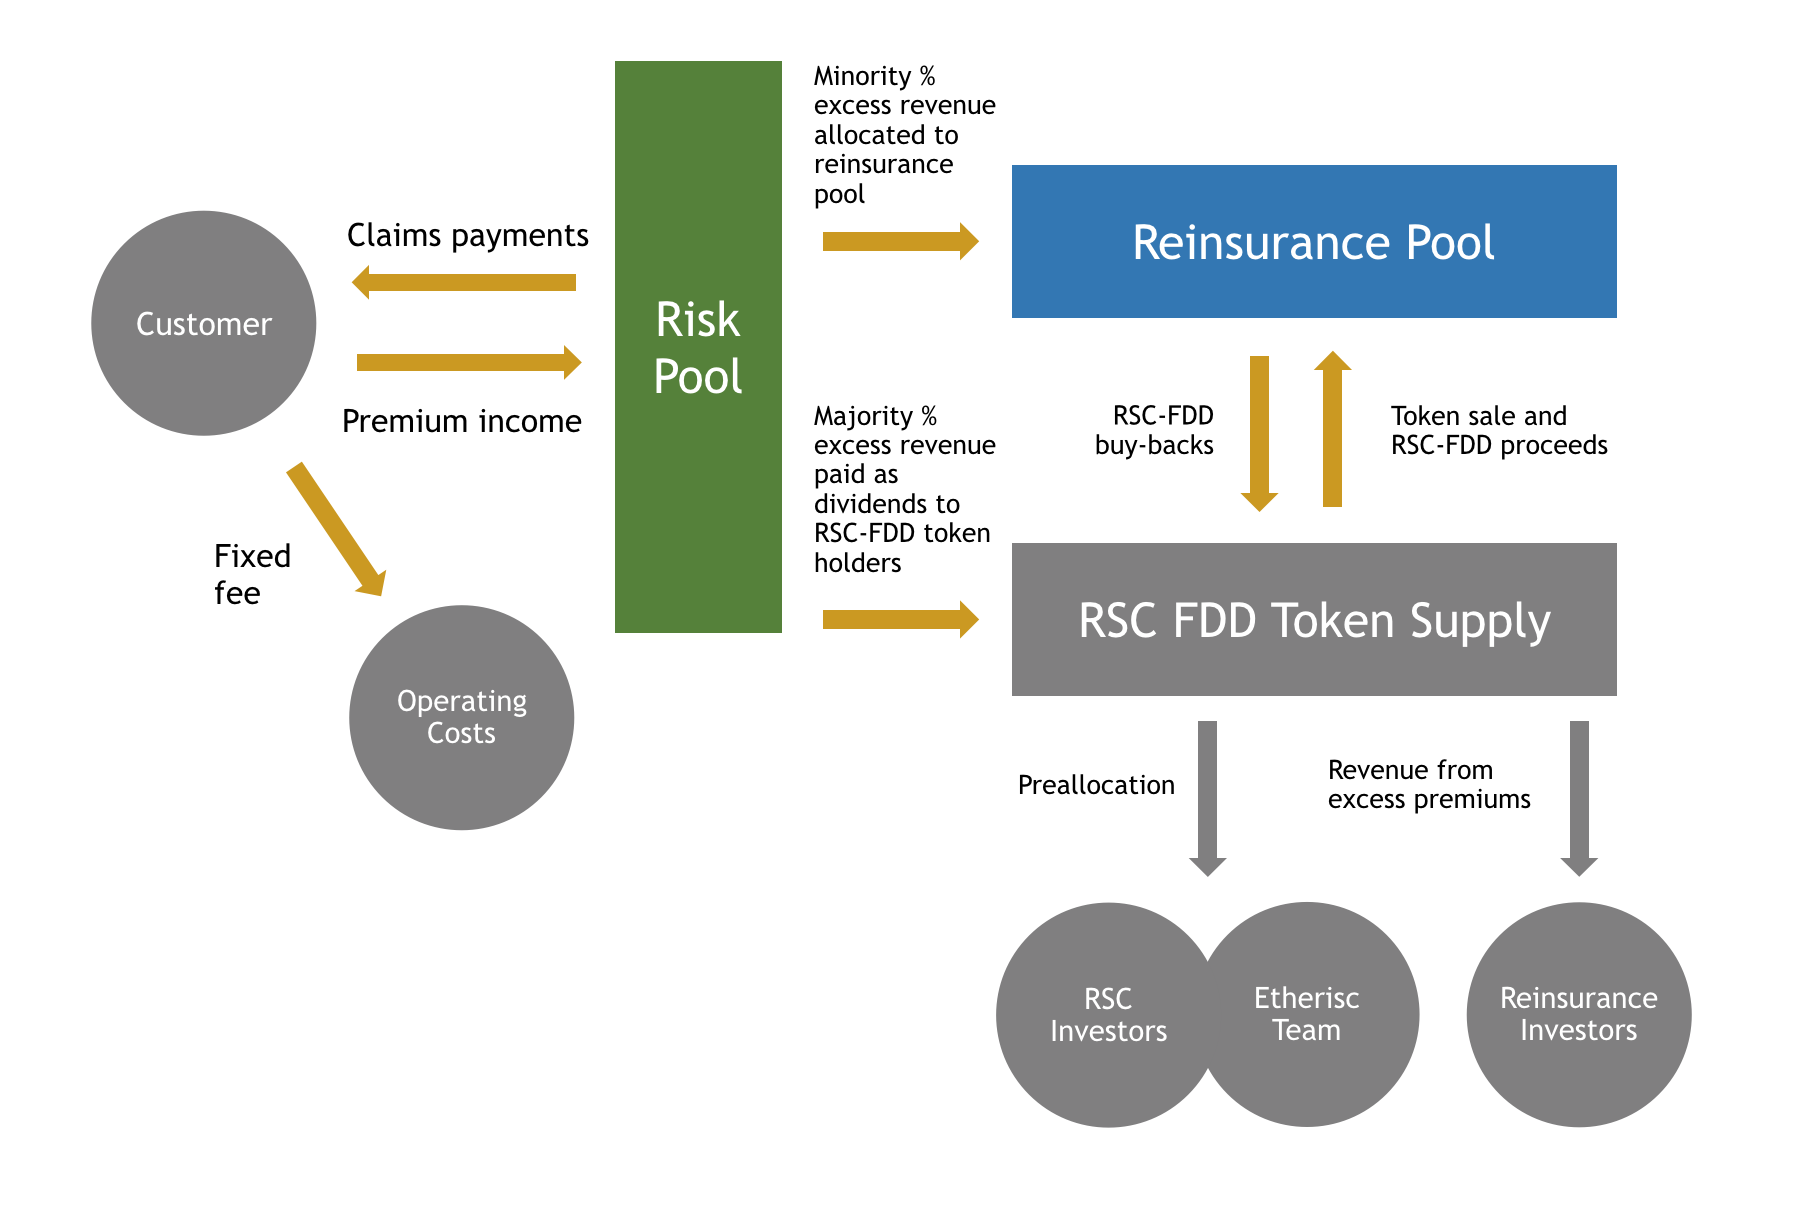
\includegraphics[scale=.5]{etheriscflows}
    \end{center}
    \caption{\footnotesize General overview of components of flight delay-based Etherisc, risk pool, reinsurance pool, and capital flows.}\label{fig1}
\end{figure}

\subsection{Risk Management for Flight Delay Insurance}

An insurance risk is a future liability for payment which occurs with a certain probability. In the case of the flight delay insurance, the probability is calculated from historical flight data. Such data is readily available from multiple trusted sources.\footnote{For instance, FlightStats (http://flightstats.com).} We assume the data quality for flight delay data to be sufficiently accurate for our purposes, considering that airlines are legally obligated to provide such data and it is highly audited by various businesses which rely on it. Insurance risks associated with flight delays are ideal for a proof of concept product, as individual premiums represent very small financial risks to consumers and investors and under normal circumstances flight delays are well-approximated by independent probability events.

A simple algorithm for premium calculation is that the average payout for claims is covered by the net premiums collected.\footnote{Net premiums are the premiums paid by the customer net of any fixed service fees.} This works well in most cases, but there can be periods where, due to statistical fluctuations, the payout is higher, sometimes even much higher than the average. This is compensated by other periods in which the payout is lower, but we have to provide enough funds that under ``most circumstances'' all payouts can be made. “Most circumstances” can be refined to a ``level of confidence'': a level of confidence of 99.9\% means that in 99.9\% of all distinct periods of time the probabilistic gross payout is smaller than the sum held in the risk pool. 

In our model, we calculate with an even higher level of confidence of 99.99\%. Put into simple words, that means that in the average, for every 10,000 years there will be one year in which the risk pool doesn’t have enough funds to pay all claims. Such a level of confidence exceeds the legal requirements; for example, in Europe, the ``Solvency II'' regulations require only a level of 99.5\% probabilistic reserve. 

Providing a risk pool at such a high level of confidence comes at a cost. Investors have to provide the capital and expect a fair return for taking the risk and binding their capital. This return is paid from excess premiums, which were not needed to pay claims, and in the end the revenue from the risk pool is designed to provide a certain surplus in excess of the net premiums collected to pay the average expected claims. 

\subsection{Risk Model Target Parameters}

Investors will ask for the key parameters of our model, therefore we provide some estimates which we will elaborate more precisely in the future. Note that all values are subject to change.
\vspace{10mm}
\begin{center}
\begin{calstable}
\colwidths{{7cm}{7cm}}
\large
\brow 
    \cell{\textbf{Parameter}} 
    \cell{\textbf{Estimate}} 
\erow
\normalsize
\brow 
    \cell{
Risk pool solvency confidence level
}
    \cell{99.99\%}
\erow
\brow 
    \cell{
Fixed service fee on premiums
}
    \cell{5 - 10\%}
\erow
\brow 
    \cell{
Target return rate on reinsurance pool
}
    \cell{5 - 10\%}
\erow

\brow 
    \cell{
Target maximum liability at launch	
}
    \cell{\$1,000,000}
\erow

\brow 
    \cell{
Target policy throughput
}
    \cell{2000 concurrent policies at\\\$500 average payout}
\erow
\end{calstable}
\end{center}



\subsection{Proposed Token Model}

We use RSC-DST to denominate the RSC tokens which are issued in the DST contract of hack.ether.camp, and RSC-FDD for the future tokens which are issued to finance the risk pool. 

Proceeds from selling RSC-DST tokens are used to back research and development and initial operational costs. RSC-DST token holders will receive RSC-FDD if funds raised exceed the funding goal and will be privileged or compensated in the sale of the RSC-FDD token.


Proceeds from selling RSC-FDD back the reinsurance pool. They are issued in a separate token sale following hack.ether.camp. After the token sale, they can be flexibly issued according to the collateralized risk volume. RSC-FDD tokens receive a revenue for providing the capital and take on the excessive risks.

%%
%% TEAM
%%

\section{Team \& Materials}

\subsection{Bios}

\subsubsection{Christoph Mussenbrock}

Christoph\footnote{https://www.linkedin.com/in/christoph-mussenbrock} has a long record of accomplishment in the cooperative banking sector in Germany. After several years on the board of a cooperative bank, he switched to the IT segment and became Chief Program Manager Credit Solutions and Chief of Strategy Development at Fiducia & GAD IT AG – one of Germany’s biggest IT Service Providers. Since 2015, he has been CEO of parcIT GmbH, one of Germany’s best-known companies specialized in risk management solutions. Due to his many years of working in the field of banking and insurance, Christoph is highly experienced in all matters concerning regulatory frameworks. He also co-founded Progeno Wohnungsgenossenschaft eG, a housing cooperative in Munich, which has successfully crowdfunded a large residential project in Munich. Christoph has a master’s degree in mathematics and wrote his thesis on formal soft- and hardware verification.

\subsubsection{Stephan Karpischek}

Stephan\footnote{https://twitter.com/kpi; https://at.linkedin.com/in/karpischek}
 is digital strategist at \textbf{disrupt consulting}\footnote{http://disrupt-consulting.com/} and has more than 20 years experience in IT businesses. He advises finance and telecom enterprises on digital strategy. In 2015 he was part of the of the UBS crypto 2.0 innovation lab at Level39 in London. Stephan has been working on digital currencies since 2008 and holds a PhD in Information Management from ETH Zürich.
 
\subsubsection{Jake Brukhman}

Jake\footnote{http://brukhman.com} is Co-Founder and Managing Partner at CoinFund,\footnote{http://coinfund.io} a blockchain technology research company and private cryptoasset investor. As part of CoinFund, Jake has studied and interfaced with a significant portion of the public blockchain startup space and has been an advisor to multiple blockchain startups. He has 9 years of experience in pure and financial technology and an avid interest in blockchain and fintech. Previously, Jake was Partner \& CTO at Triton Research, a technical product manager and engineer at Amazon.com, and spent five years as a financial technologist at Highbridge Capital Management and as a quantitative researcher and trader at Kohera. Jake studied computer science and mathematics at Rutgers University, New Brunswick and the Courant Institute of Mathematical Sciences at NYU.

\subsubsection{Nuno Brito Lopes}

Nuno is the sole proprietor of lopezi.com which, in collaboration with an extended network of professionals, provides a wide range of Digital Design and IT Services. Before settling in central Europe, he worked in the Iberian Peninsula and in the Middle East across multiple industries, for companies such as Siemens, Huawey, E.ON and Telefonica’s O2. He has a BSc in Visual Information Technologies by the University of Coimbra. With management and strategy experience he is also the former CTO of inCare GmbH. 

\subsubsection{Renat Khasanshyn}

Founder and CEO of Altoros\footnote{http://altoros.com}, and Venture Partner at Runa Capital. Altoros is a 250+ people strong consultancy helping its clients turn latest advancements in blockchain into competitive advantage. For example, it has designed architecture and built PoCs for canonical use cases of blockchain: bond issuance and trading, catastrophe bonds, insurance fronting, reinsurance, clearing and settlement of credit default swaps. In the Etherisc Hackathon team, Renat works as a front-end web developer, focusing on UI/UX of conversion mechanisms and the risk marketplace.

\subsubsection{Ron Bernstein}

Ron is the Co-Founder and Managing Director of AugmentPartners Limited; a software consultancy related to digital technology and decentralized trading, and an advisor to The Augur Project; a decentralized prediction market. Ron has traded commodity futures and options for more than 25 years on the trading floors in New York and London. Fascinated by the convergence of the Internet, sports betting, and prediction markets; Ron founded Intrade.com in 2000 and Tradesports.com in 2003. Recent development of digital currencies, blockchain, and especially decentralized software systems fuels Ron’s interest in prediction markets and how they may be applied in the real world to benefit everyday life.

\subsection{Past Milestones}

\begin{itemize}
    \item Flight Delay App tested at Devcon2.\footnote{https://fdd.etherisc.com/}
    \item Lessons learned from Flight Delay App alpha test.\footnote{https://medium.com/the-future-requires-more/flight-delay-dapp-lessons-learned-a59e4e39a8d1}
    \item Flight Delay press on CryptocoinNews.\footnote{https://www.cryptocoinsnews.com/blockchain-disrupt-air-travel-insurance-flightdelay/}
    \item CoinFund Q\&A with Etherisc founders.\footnote{https://www.youtube.com/watch?v=baRg0iCPrK8}
    \item Etherisc wins Blockchain Startup Contest\footnote{http://ethnews.com/winners-of-the-blockchain-startup-contest-announced-etherisc-and-status}. 
    \item Blockchain Startup Contest presentation video.\footnote{Winner Blockchain Startup Contest 2016
Presentation video}
    \item Etherisc becomes most funded started at hack.ether.camp.\footnote{https://www.youtube.com/watch?v=FYXn7qtp0v8}
\end{itemize}

\subsection{Github}
The Etherisc Github repository for hack.ether.camp may be found here:
\begin{verbatim}
    https://github.com/etherisc/hackathon
\end{verbatim}

\subsection{Chatroom}
The Etherisc public Gitter channel may be found here:
\begin{verbatim}
    https://gitter.im/etherisc/Lobby
\end{verbatim}

\newpage
\LARGE\textbf{APPENDIX}\normalsize
\appendix

\section{Credit Risk Model}

\subsection{Abstract}

This is a technical addendum to the Etherisc\footnote{http://etherisc.com} decentralized insurance whitepaper, presented at the EtherCamp Virtual Accelerator (http://hack.ether.camp). In this work, we develop a simple probability model for a parametric insurance pool with variable claim payouts and variable probabilities of insurable events. We present one methodology for calculating premiums. We also suggest avenues for employing this model in a real-time context of a portfolio that continuously underwrites claims. Finally, we present a Python simulation which puts our modeling methodology into practice against actual data for insurable flight delays.}

\subsection{Overview}

In this section, we describe the desirable properties of a basic credit risk model for decentralized insurance with a minimum viable set of features that can enable the proof of concept Etherisc application. In general, insurance works by selling policies which cost the purchaser a premium in exchange to an entitlement to a payout in the case of some \textit{insurable event}. The occurrence of the event and subsequent automated payout is referred to as a \textit{claim}. The Etherisc demo application focuses on the case of flight delays, but in our model we do not make any assumption about the specific nature of the event with an eye to expanding our insurance offering to different markets.

An insurance risk pool underwrites policies by taking on some maximum liability in the form of credit for potential claims, and collateralizing the portfolio with a smaller amount of capital to cover the capital outflow due to claims with a reasonable confidence level. If the portfolio experiences a capital outflow of claims which exceeds the collateralization of the risk pool, the risk pool becomes insolvent. This problem of excess risk management is addressed by the Etherisc whitepaper and its decentralized reinsurance market based on cryptographic tokens.

We target the following mathematical properties in our model of an insurance risk pool:

\begin{enumerate}
\item The portfolio should be able to reasonably model insurable events as independent (and uncorrelated) random variables.
\item The model should be able to provide distinct probabilities of each individual event as parameters.
\item The portfolio should be able to underwrite policies for an arbitrary payout amount.
\item The model should be able to parametrize the probability of solvency of the portfolio at an arbitrarily high confidence level.  
\end{enumerate}

In modeling insurance, correlation analysis of events plays a key role in achieving highly realistic models but significantly increases model complexity. For the purposes of our proof of concept product, we assume independence of insurable events and offload the risk due to error to our reinsurance market (covered in the Etherisc whitepaper). We recognize the importance of correlation analysis and future efforts will focus on developing more granular modeling methodologies. Note that this model's ability to underwrite payouts of arbitrary size is crucial because it enables the risk pool underwrite multiple policies pertaining to the same event without requiring a model based on correlated random variables.

In general, we also desire that our model outputs should cover the gamut of relevant financials that might be useful in constructing a smart contract\footnote{Decentralized insurance rests on the idea of a decentralized implementation on a smart contract platform such as Ethereum. See: http://ethereum.org.} which manages the insurance pool: (i) the total liability of the credit portfolio; (ii) the required collateralization of the risk portfolio; (iii) at least one plausible method for calculating premiums commensurate with event probabilities and payouts; and (iv) an expectation and spread for the revenue of the portfolio (ideally, non-negative).

Finally, our model should be straightforward to calculate (or estimate). In the following section, we develop the mathematics for a model which conforms to the properties above.

\subsection{Probability model}

Let us assume that our risk pool portfolio contains $n$ policies which are insuring against $n$ insurable events, modeled as independent but not necessarily identically distributed random variables $X_i$ $(i=1,\ldots,n)$. Suppose that $P^*_i$ $(i=1,\ldots,n)$ is a fixed set of desired payouts where $P^*_i$ corresponds to the policy $i$. Furthermore, suppose that $X_i\in\{0,1\}$ are Bernoulli random variables with event probability $p_i$ $(i=1,\ldots,n)$. That is, $P(X_i = 1) = 1 - P(X_i = 0) = p_i$ for $i = 1,\ldots,n$. 

The \textit{total liability} $L$ of the portfolio is the sum of all payouts the portfolio is underwriting, and we define 
% %
% %
   $$L(n) := \sum_{i=1}^n P^*_i.$$
% %
% %
% We are interested to find the \textit{required collateral} $C(n)$, that is, the amount of capital the portfolio will hold to handle capital outflows due to claims. Typically, $C(n)/L(n)<1$, reflecting the fact that the portfolio is taking on credit risk. Our goal is to keep enough collateral in the portfolio to be able to pay a reasonably expected number of policy claims. We define the total capital outflow due to claims as
% %
% %
%   $$X:=\sum_{i=1}^n X_i P_i^*.$$ 
% %
% %
$X$ is a random variable that has a non-trivial distribution which is the weighted sum of Bernoulli variables with non-uniform probabilities. Let us define $\pi$ to be the desired confidence level (probability) of portfolio solvency, and we note that typically $\pi$ will be high ($\pi\approx 1$). Let $F_X$ be the cumulative distribution function of $X$. Our model is then defined by setting the required collateral $C$ to the $\pi$-percentile probable capital outflow due to claims:
% %
% %
\begin{equation}
    \label{model}
    C(n) = F_X^{-1}(\pi).
\end{equation}
% %
% %
Let us now to turn to calculating the set of premiums $P_i$ $(i=1,\ldots,n)$. For one, we must have that $\sum_{i=1}^n P_i = C(n) = F_X^{-1}(\pi)$, but we are free to choose how to distribute the claim costs among policies. While there are multiple ways to distribute the collateralization cost, we choose a method that has naturally desirable properties: (i) the premium $P_i$ should be proportional to the payout $P_i^*$ (intuitively, the higher the payout of a policy, the more the upfront premium cost); (ii) the premium $P_i$ should be proportional to the insurable event probability $p_i$ (intuitively, the lower the probability of the event, the cheaper the premium). To achieve this relationship, set
% %
% %
     $$P_i := \frac{p_iP_i^*}{\sum_j p_jP_j^*} F_X^{-1}(\pi)$$
% %
% %
and it is clear that (\ref{model}) holds. Moreover, it is easy to check that $P_i \to 0$ as $\pi \to 0$ and $P_i\to\infty$ as $P_i^*\to\infty$ as required. If we find that at a small $n$ our premiums are too expensive, we have the option of reducing premiums with some initial subsidy capital seeded into the risk pool; however, we will not pursue the mathematical details of this extension as we believe premiums will already be sufficiently small.

A straightforward calculation shows that the expected value and standard deviation of $X$ are given by
% %
% %
  $$E(X) = \sum_{i=1}^np_iP_i^*\ ;\ \ \sigma_X = \sqrt{\sum_{i=1}^np_i(1-p_i)(P_i^*)^2}.$$
% %
% %
\begin{figure}[H]
    \begin{center}
        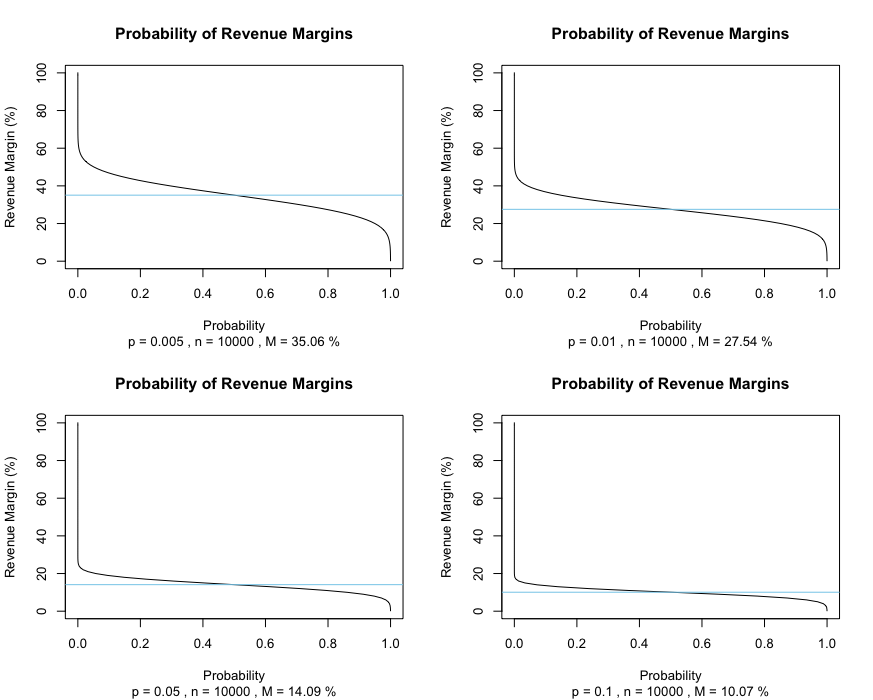
\includegraphics[scale=.5]{margins}
    \end{center}
    \caption{\footnotesize Probability distributions of revenue margins given different values of average event probability $p$. $M$ is the \textit{revenue margin}, the difference between capital outflows due to claims and the collateral $C$, divided by $C$.}\label{fig1}
\end{figure}
% %
% %
We now demonstrate that, given collateralization, our model produces a non-zero expectation of revenue with $\pi$-confidence. To show this, let us define the revenue $R$ as the excess capital remaining in the pool after capital outflows due to claims
% %
% %
    $$R(n) := C(n) - X(n)$$ 
% %
% %
and note that $R(n)>0$ with probability $\pi$. (Observe that $E(R)=E(C)-E(X)=F_X^{-1}(\pi)-F_X^{-1}(.50)$ and because of our self imposed constraint that $\pi \approx 1 >.50$ we have $E(C)>E(X)$.) More explicitly, note that the mean and standard deviation of revenue under this model is given by:
% %
% %
$$E(R) = F_X^{-1} - \sum_i p_i P_i^*\ ;\ \ \sigma_R = \sqrt{\text{var}(C) + \text{var}(X)} = \sigma_X.$$
% %
% %
We now summarize the inputs and outputs of the Etherisc credit risk model.

\subsubsection{Model inputs}
\begin{enumerate}
    \item A vector of insurable event probabilities $\mathbf{p}=\left<p_i\right>$, $(i=1,\ldots,n)$.
    \item A vector of desired payouts $\mathbf{P^*} = \left<P_i^*\right>$, $(i=1,\ldots,n)$.
    \item A confidence level for portfolio solvency $\pi$, where $.5 < \pi < 1$.
\end{enumerate}

\subsubsection{Model outputs\label{outputs}}

\begin{enumerate}
    \item \textbf{Total Liability.} Total portfolio liability is given by $$L(n) := \sum_i P_i^*$$.
    \item \textbf{Collateral.} Required minimal collateral is given by $$C(n) := F_X^{-1}$$.
    \item \textbf{Excess Liability.} The excess portfolio liability on offer to a reinsurance market is $$\tilde{L}(n) := L(n) - C(n)$$.
    \item \textbf{Premiums.} A vector of premiums corresponding to the payouts $\mathbf{P^*}$, given by $$\mathbf{P}:=\left<\frac{p_iP_i^*}{\sum_j p_j P_j^* }F_X^{-1}(\pi)\right>.$$
    \item \textbf{Capital Outflow.} The expected capital outflow due to claims is $E(X)=\sum_i p_iP_i^*$. The standard deviation of capital outflow due to claims is $$\sigma_X =  \sqrt{\sum_{i=1}^np_i(1-p_i)(P_i^*)^2}$$.
    \item \textbf{Expected Revenue.} The expected revenue for the portfolio is $E(R) = C(n) - \sum_{i=1}^n p_i P_i^*$. The standard deviation of revenue is $$\sigma_R = \sigma_X = \sqrt{\sum_{i=1}^np_i(1-p_i)(P_i^*)^2}$$.
\end{enumerate}

\subsubsection{Properties}

We now summarize the general mathematical properties of the credit risk model we have described.

\begin{enumerate}
    \item The total liability of the risk portfolio increases with the number $n$ of policies, but the required collateralization (that is, $C(n)/L(n)$) tends to decrease with $n$.
    \item Premiums become less expensive as the number of policies grows; that is, $P_i\to 0$ as $n\to\infty$. Premiums are also proportional to the corresponding payout and insurable event probability under the premium calculation we have described.
    \item In general, the premiums can be calculated using any algorithm that distributes the required collateral $C$ among $n$ policy holders. A reasonable framework for this calculation is that $$P_i = kp_iP_i^*$$ should hold for the $i$-th policy for some constant $k > 0$.
    \item Expected revenue is inversely proportional to the insurable event probabilities and standard deviation of revenue decreases as probabilities decrease. Unsurprisingly, the variance in revenue is the variance of capital outflows due to claims.
    \item As demonstrated in Figure 1, revenue margins decrease with higher efficiency of the system (higher $n$) and lower average event probability $p$.
\end{enumerate}

\subsection{Discussion of practical applications}

In practice, an insurance risk pool operates continuously: it has some number of valid policies currently being underwritten and creating liability as well as incoming requests for new policies to be underwritten. In a practical context, the pricing of premiums is directly related to marginal changes of the required collateralization $C$ of the risk portfolio.

For instance, suppose the current state of the portfolio requires collateral $C$, but a new policy is requested against a new or existing event. Recalculation of the model will result in a new required collateralization $C'$ which must be maintained for $\pi$-confidence of solvency (and as the portfolio is taking on more risk, $C'>C$). Since the standing premiums in the portfolio have already been remitted, their values cannot be changed. Thus the fair price of a new premium is $\Delta C := C' - C$, guaranteeing that $\pi$-confidence is maintained.

In general, the price of a premium should correlate positively with both the payout and the probability of the insurable event: that is, $P_i = kp_iP_i^*$ for some constant $k>0$. In practice, $\Delta C$ may exceed this "expected" baseline premium, especially when the portfolio is small, and so subsidization of the risk pool may be required to bring premiums to expected levels. This scenario is covered in the Etherisc whitepaper through revenue reallocation.

\subsection{Model estimation}

\subsubsection{Calculation}

The core complexity of the model estimation algorithm is the non-triviality of the distribution of random variable $X$. In order to find $C$, we must estimate $F_X^{-1}(\pi)$ which is computationally difficult to do directly. Instead, we take an estimation approach by taking some large $N$, and simulating $N$ random outcomes for the value of $X$, followed by running a known percentile estimation algorithm on the random outcome for the $\pi$-percentile. The rest of the model outputs follow by straightforward calculation based on Section \ref{outputs} above.

\subsubsection{Python simulation}

The model described above is implemented as a Python simulation. Please see:
\begin{verbatim}
    https://github.com/etherisc/hackathon/tree/master/etherisc-simulator
\end{verbatim}

\subsubsection{Example outputs}

The following simulation demonstrates a calculation of the insurance model on a set of 60 real flights given actual flight delay estimates from FlightStats. In this calculation, we have set a fixed payout of \$250 for each policy. The model has determined the total liability $L$ of the portfolio to be \$15,000 and a required collateralization $C=\$3,750$, a $25\%$ collateralization of the portfolio. The expected revenue $R=\$2,337.37$ with a standard deviation of $\$561.27$.

As discussed, note that the theoretical premiums displayed below are different from what would be provided to customers. In general, the premiums can be adjusted lower or higher using subsidization of the risk pool. In practice, premiums will also include additional fixed service fees.

\begin{verbatim}# Etherisc insurance calculation

      n:   60
      mu:  1412.63
      sd:  561.27
      L:   $15000.00
      C:   $3750.00
      %:   25.00
      r:   4.00
      R:   $2337.37
    
                     prob    premium  payout
DL_762_ATL_MDW   0.018182  12.066488     250
WN_349_RIC_ATL   0.022727  15.083110     250
WN_349_ATL_CMH   0.022727  15.083110     250
WN_203_BNA_SAT   0.026316  17.464685     250
DL_780_ATL_CVG   0.040000  26.546313     250
DL_762_MDW_ATL   0.040000  26.546313     250
KL_724_HAV_AMS   0.040816  27.088050     250
DL_132_TPA_DTW   0.046512  30.867805     250
SK_904_EWR_ARN   0.048387  32.112468     250
DL_160_MSP_AMS   0.048387  32.112468     250
DL_132_DTW_AMS   0.052632  34.929329     250
WN_203_MDW_BNA   0.052632  34.929329     250
AC_36_BNE_YVR    0.053571  35.553061     250
KL_642_JFK_AMS   0.064516  42.816613     250
DL_160_IND_MSP   0.064516  42.816613     250
DL_1527_ATL_FLL  0.065574  43.518511     250
DL_476_JFK_BCN   0.066667  44.243829     250
WN_349_CMH_MCO   0.068182  45.249369     250
AA_1033_DFW_RSW  0.073171  48.560297     250
DL_2452_ATL_RIC  0.075472  50.087360     250
WN_203_ABQ_BWI   0.081081  53.810073     250
DL_337_ATL_NAS   0.083333  55.304776     250
DL_1527_FLL_ATL  0.084746  56.242159     250
DL_142_LAS_SEA   0.093023  61.735571     250
AA_66_SFO_JFK    0.096774  64.224937     250
SK_903_ARN_EWR   0.096774  64.224937     250
LA_3010_BOG_MDE  0.098361  65.277789     250
DL_2452_RIC_ATL  0.098361  65.277789     250
DL_72_MCO_ATL    0.098361  65.277789     250
YV_6273_IAH_ELP  0.100000  66.365763     250
DL_54_ATL_LOS    0.100000  66.365763     250
EV_5230_ATL_BTR  0.111111  73.739715     250
F9_1539_ATL_PHX  0.111111  73.739715     250
WN_258_GSP_ATL   0.111111  73.739715     250
WN_258_PHL_TPA   0.111111  73.739715     250
LA_800_AKL_SCL   0.112903  74.929082     250
DL_72_ATL_AMS    0.112903  74.929082     250
NZ_29_IAH_AKL    0.113636  75.415629     250
EV_5597_LFT_ATL  0.114754  76.157406     250
EV_5597_ATL_LFT  0.114754  76.157406     250
KL_624_ATL_AMS   0.117647  78.077347     250
EV_5230_ATL_FAY  0.117647  78.077347     250
EV_5230_FAY_ATL  0.117647  78.077347     250
KL_678_YYC_AMS   0.118644  78.739020     250
OO_4568_SLC_PHX  0.120000  79.638900     250
DL_907_DTW_RDU   0.120000  79.638900     250
DL_54_IAD_ATL    0.128205  85.084289     250
LA_800_SYD_AKL   0.129032  85.633220     250
AA_83_JFK_LAX    0.129032  85.633220     250
KL_652_IAD_AMS   0.129032  85.633220     250
KL_606_SFO_AMS   0.129032  85.633220     250
QR_755_DOH_ATL   0.131148  87.037061     250
WN_203_BWI_MDW   0.131579  87.323337     250
DL_477_BCN_JFK   0.133333  88.487664     250
HA_444_BNE_HNL   0.137931  91.538975     250
DL_476_LAX_JFK   0.142857  94.808205     250
DL_675_NAS_ATL   0.145161  96.337365     250
LA_3508_BOG_CUN  0.145161  96.337365     250
JJ_8000_GRU_BOG  0.145161  96.337365     250
NZ_10_AKL_HNL    0.147059  97.596702     250
\end{verbatim}
\begin{figure}[H]
    \caption{\footnotesize Example calculation on a 60-policy insurance portfolio using actual flight delay data.}\label{fig2}
\end{figure}

\section{Crowdsale [Under Review]}

The creation and distribution of blockchain-based cryptographic tokens has quickly become the de facto methodology for funding software projects building open protocols.
According to Smith + Crown, since January of 2013 until early December 2016, approximately \$270 million has been committed to decentralization software projects using cryptographic token economies and fundraising for project development. Anecdotally, there were approximately 40 publicized token offerings in 2016, compared to 17 traditional IPO’s in the Technology sector during the same time frame. The pace is accelerating. According to ICORATING.com, there are approximately 10 projects currently in the planning or execution phase for decentralized crowdfunding, and new projects are being announced on a weekly basis.

Because of the volume and interest in these new models, the intense scrutiny of the economics involved by a “vocal” crypto-community, and the breadth of participation and observational commentary, a basis for “best practices” for token distributions is emerging.

Etherisc is committed to providing complete transparency for its token offering and distribution methodology and to adhere to best practices being followed today by the blockchain community at large.

\subsection{Token Distribution Best Practices}

\subsubsection{Prerequisites}

\begin{enumerate}
    
    \item The token should have a defensible use case within the model or economics of the business.
    \item The project must utilize open source software and publish the relevant code and documentation in advance of initial token distribution.
\end{enumerate}

\subsubsection{Information and Mechanics}

\begin{enumerate}
    \item The project must clearly communicate the token/equity structure including (1) the total (lifetime) supply of available tokens (including inflationary and/or deflationary factors); (2) the reasoning for the initial token allocation available for distribution, (3) the method of initial token distribution, 
    and (4) the ability for future fungibility of the token.
    
    \item The project should cap the value of initial contributions based upon a demonstrated and budgeted need in relation to total available lifetime supply (i.e. traditionally known as “market cap”) AND considerate of the funding amount desired from the distribution derived from a detailed project plan and roadmap.
    
    \item There should be a logical relationship between project governance and pro rata token ownership. Governance criteria and methodology should be logical, inclusive, meaningful, and intuitive.
    
    \item The project should fully disclose the Founders, Advisors, and team allocation in advance of the distribution, and this allocation as a category should include some aspect of “vesting” of ownership over time for key personnel.

    \item The project should utilize a “level-field” pricing mechanism and clearly communicate if earlier risk takers are compensated extra-ordinarily.
    
    \item There should be a definitive start and end date for the initial distribution phase with minimized economic incentive for early participation in this distribution phase (as business risks during this phase are all being assumed at essentially the same time).
    
    \item The project should provide an intuitive UI/UX for crowdsale participation, and attempt to maximize breadth of participation.

    \item The project should utilize a non-proprietary blockchain for distribution and “proof” of distribution, with limited options for permitted “buy-in” currencies.


    \item The project should establish and publish guidelines for the minimum amount of commitment required to undertake the token distribution as well as a process for the return of commitments upon failure to achieve minimum project thresholds.

\end{enumerate}

\subsubsection{References}

\begin{enumerate}
    \item Fred Ehrsam, Coinbase, August 2016.\footnote{https://blog.coinbase.com/app-coins-and-the-dawn-of-the-decentralized-business-model-8b8c951e734f#.wnj6cp2fp}

    \item Demian Brener, Smart Contract Solutions, August 2016.\footnote{http://www.coindesk.com/tokens-crowdsales-startups/}

    \item William Mougayar, November 2016 and earlier references.\footnote{http://startupmanagement.org/2016/11/24/how-to-evaluate-an-initial-cryptocurrency-offering-ico/}
    
    \item Zenel Batagelj, Iconomi, November 2016.\footnote{https://medium.com/iconominet/ico-2-0-what-is-the-ideal-ico-ee9d285a8939#.bhilra2dp}

    \item General news, research and analysis of cryptoeconomics and ICO research from Smith + Crown.\footnote{https://www.smithandcrown.com/icos/}

    \item Jake Brukhman, CoinFund, July 2016.\footnote{https://blog.coinfund.io/blockchain-investments-and-the-new-problem-asset-for-conventional-vcs-b65bfc7ca75}
\end{enumerate}

%%
%%
%%
%%
%%
%%
%%
%%
%%
%%
%%
%%
%%
%%
%%
%%

\section{Security and Formal Verification [Under Review]}

Recent events involving “TheDAO” hack, various hacks of exchanges, and cryptocurrency wallet vulnerabilities, [citation needed] have shown that security is a top priority for decentralized projects. We plan to take security very seriously and implement a number of active and passive strategies for establishing the secure operation of the Etherisc system.

Besides classical IT-related security measurements like use of coding best practices, code reviews, security audits, and both active and passive network security we will especially dive in the evolving field of formal verification.


Formal verification of smart contract will be the key feature to provide us with a level of security unreachable with simple test-driven development (TDD).

We are working with the Munich team of Prof. Dr. Helmut Schwichtenberg, a well-known researcher in the field of formal verification. The team of Prof. Schwichtenberg has build the minlog system (http://minlog-system.de), a minimal-logic theorem prover capable of extracting programs out of existential proofs (a proof of x,y z:z=x+ycan be used to generate a program to compute x+y). Numerous case studies suggest that this will be a promising path towards a thorough, end-to-end verification of smart contracts, the most sensible parts in the chain of work.


One of the main obstacles for formal verification is the lack of clear specification to a given implementation of a certain use case. We will tackle this problem by introducing a stack of abstractions. Every subsequent level interprets or implements the higher level, and then we prove the correctness of the implementation in relation to the specification. After finishing the whole stack, we have a thorough proof from the highest level down to the lowest level, which could be bytecode for example.

To illustrate this, we propose the following stack of abstraction:

\textbf{TODO: table}

Of course, a complete chain of proof will be difficult and maybe a work of years. We will therefore start with proofs levels 1, 2, and 3, while proofs of levels 3, 4, and 5 will be a long-term project available to the whole community.

\section{General Regulatory Considerations [Under Review] \label{regulatory}}

Banking and insurance are among the  most regulated economic fields. Over-regulation  precludes many promising business models and introduces expensive frictions whose cost is ultimately transferred  to the end consumer.


Among other things, regulatory requirements are designed to protect consumers. Banks and insurance companies require licenses to protect consumers from unscrupulous companies. Regulatory authorities have extensive monitoring rights, and banks and insurance companies are required to have a sufficient capital base. This is all good and a reasonable tool to protect consumers. The financial crises of the past few decades have however shown that rules and regulations often prove ineffective. Companies were often “one step ahead” and successful in finding loopholes in existing regulation (a good example would be Lehman Brothers).

This said, we are aware that regulation and consumer protection on the Blockchain require new ways of thinking. On the Blockchain, we cannot enforce consumer protection via external conditions and legal frameworks. Although there is no absolute anonymity and you can comprehend monetary flows with some effort, central regulation contradicts the fundamental principles of a decentralized blockchain. The Blockchain is basically a self-regulating system.

We therefore believe that the mechanisms for effective consumer protection on the Blockchain have to be reinvented (a good example of such protection is the "split" function of DAO. It will be interesting to follow the further development of this and similar schemes.)
We do not oppose consumer protection, on the contrary! Protection of all users of the blockchain  is vital for the evolution of the network. Only if the users – and  especially the non-tech savvies – can rely on fairness and safeguard of their interests, this technology can find its way to bigger masses.

These mechanisms must be such as to  correspond with the nature of the Blockchain. We can therefore only use decentralized and autonomous protective mechanisms, thus ultimately self-regulating mechanisms that are proposed and implemented by the users of the blockchain itself.[SK1] 

Yet it is of absolute importance that the development of these mechanisms will be monitored by  the established supervisory authorities with a friendly attitude. Otherwise, it is possible that the authorities will try to impose their rules on the Blockchain in ignorance of the details. Since by design and architecture, the Blockchain is largely immune to external influence, regulators will have no choice but to limit access to the Blockchain, crushing all further evolution of  Blockchain technology.

Etherisc works very closely with German and European regulatory authorities, and we will actively use our existing network to create an understanding on the part of the authorities of the particularities of this new technology; etherisc will be right at the interface between Blockchain and the traditional financial markets.

We will take great care to ensure that no entity or company comes into existence which could be formally interpreted as an "insurance company" or "bank". Therefore, we interpret all Smart Risk Contracts as consensual agreements between individuals, installed as software on the Blockchain for the control of cash flows. This is the blockchain analogue of the "freedom of contract" under civil law. We as Etherisc merely act as a consultant, provide templates for smart contracts, and assist the parties in negotiating fair premiums.

Etherisc does not advise any party to enter into such an agreement; it is also not allowed  to incentivize partners to conclude contracts. All these criteria are fulfilled by the autonomous risk sharing platform. With respect to the regulatory institutions, Etherisc will accept responsibility only for the optimal calculation of risk premiums.

\section{Related Work \& References [Under Review]}

\subsection{Other decentralized insurance projects}

\textbf{InsurETH} (Thomas Bertani, Kristina Butkut, Francesco Canessa) InsurETH was the winning project at the “Hack the Block” hackathon at London Fintech Week in late 2015. To our knowledge it was the first project to recognize the great fit for flight delays as an ideal use case for parametric insurance in a smart contract. Thomas and the team at Oraclize have supported the Etherisc team from its inception. The Flight Delay Dapp uses Oraclize to channel flight data into the FDD smart contract. We are thankful and happy to have their support.

\begin{itemize}
    \item Website: http://insureth.mkvd.net/
    \item Presentation slides: http://mkvd.s3.amazonaws.com/apps/InsurEth.pdf
    \item Github repository: https://github.com/makevoid/insurETH\_trains 
\end{itemize}


\textbf{Dynamis} (Joshua Davis) Joshua has shared his vision on peer-to-peer insurance on the blockchain and was an early inspiration for us to create decentralized insurance applications. At Etherisc we would love to see this vision of a peer-to-peer insurance marketplace become reality. We are working on it and are thankful for this groundbreaking work.

\begin{itemize}
    \item Whitepaper: http://dynamisapp.com/whitepaper.pdf
\end{itemize}

\textbf{Inchain} Inchain has been among the first major projects to raise funds for a blockchain insurance application in a token sale. We were among the early supporters of their good idea and would have loved to see them succeed and develop insurance for crypto assets. Unfortunately, their funding goal was not reached. 

In contrast to Inchain, we can demonstrate a fully functional prototype of a parametric insurance, you can try our prototype at https://fdd.etherisc.com. We have developed and published a risk model, which already works nicely in simulations, see Appendix A: Credit Risk Model.

\begin{itemize}
    \item Website: https://ico.inchain.io 
\end{itemize}

\textbf{ChainThat}

\begin{itemize}
    \item Website: http://chainthat.com
    \item Press: http://www.the-digital-insurer.com/blog/insurtech-the-insurance-market-chainthat-21st-century-coffee-house-on-blockchain/
\end{itemize}

\textbf{BlockSure} https://blocksure.com

\textbf{Town Crier Demo} https://twitter.com/initc3org/status/758662838802083840

\textbf{WeTrust} http://wetrust.io

\textbf{BitPark} https://bitpark.net

\subsection{Industry research \& development}

\begin{itemize}
    \item Allianz Catastrophe Bonds is testing three different blockchain technologies.\\ http://www.coindesk.com/allianz-blockchain-smart-contracts-boost-catastrophe-bond-trading
    \item B3I initiative: Aegon, Allianz, Munich Re, Swiss Re and Zurich join forces to explore blockchain.\\https://www.munichre.com/en/media-relations/publications/company-news/2016/2016-10-19-company-news/index.html
    \item http://www.zhongtuobang.com/site/blockchain
    \item Michael Mainelli, Long Finance, Chain of a Lifetime.\\ http://www.longfinance.net/lf-research.html?id=903
    \item Michael Mainelli and PwC, Chain Reaction\\ http://www.longfinance.net/lf-research.html?id=903
    \item McKinsey report.\\ http://www.mckinsey.com/industries/financial-services/our-insights/blockchain-in-insurance-opportunity-or-threat
    \item Deloitte, Blockchain in health and life insurance.\\ https://www2.deloitte.com/us/en/pages/life-sciences-and-health-care/articles/blockchain-in-insurance.html
    \item "Analysis of aircraft arrival delay and airport on-time performance." Yuqiong Bai.\\ http://etd.fcla.edu/CF/CFE0001049/Bai\_Yuqiong\_200605\_MS.pdf
    \item Collin Thompson.\\ https://medium.com/@collin\_thompson/insurance-the-blockchain-and-the-sharing-economy-re-imagining-insurancetech-with-p2p-social-8211e922fa79
    \item David Siegel. Insurance on the Blockchain. In his article for the ConsenSys blog David coins the term “insure-bits” to describe the tokenization of risks. The following discussion about insurance on the blockchain in the 2030 blockchain business community brought together Stephan and Christoph to work on the Flight Delay Dapp and later form the founding team of Etherisc.\\https://media.consensys.net/2016/07/19/insurance-on-the-blockchain/\\https://medium.com/@pullnews/insurance-on-the-blockchain-eb06fe23730e
    \item https://techcrunch.com/2016/10/29/blockchain-is-empowering-the-future-of-insurance/ 
\end{itemize}




\end{document}
